%\addcontentsline{toc}{chapter}{Development Process}
\chapter{Design}

%You should concentrate on the more important aspects of the design. It is essential that an overview is presented before going into detail. As well as describing the design adopted it must also explain what other designs were considered and why they were rejected.

%The design should describe what you expected to do, and might also explain areas that you had to revise after some investigation.

%Typically, for an object-oriented design, the discussion will focus on the choice of objects and classes and the allocation of methods to classes. The use made of reusable components should be described and their source referenced. Particularly important decisions concerning data structures usually affect the architecture of a system and so should be described here.

%How much material you include on detailed design and implementation will depend very much on the nature of the project. It should not be padded out. Think about the significant aspects of your system. For example, describe the design of the user interface if it is a critical aspect of your system, or provide detail about methods and data structures that are not trivial. Do not spend time on long lists of trivial items and repetitive descriptions. If in doubt about what is appropriate, speak to your supervisor.
 
%You should also identify any support tools that you used. You should discuss your choice of implementation tools - programming language, compilers, database management system, program development environment, etc.

%Some example sub-sections may be as follows, but the specific sections are for you to define. 

\section{Overall Architecture}

MVC - for ease of testing, scalability, separation of concerns, maintainability through familiarity(people know mvc and what to expect), maturity of supporting technologies

3-tier based approach to data layer / service / presentation stuff that may not entirely fit with the mvc pattern

\section{Framework and Programming Language}

The sheer range of MVC frameworks available to developers is incredible and the decision of which to use is potentially difficult. It was not within scope to review all the available choices 


\section{Tools and third-party services}
\subsection{Intellij}
\subsection{Git and Github}
\subsection{Jira}

Jira \cite{jira} in an issue tracking and project management tool provided by Atlassian, an Australian software company. It is an industry leading product used by many companies for tracking their projects and the issues within them. Its use on this project was in support of the agile approach to project development, allowing the specification of user stories, development tasks and their inclusions within configurable sprints or development iterations. Figure \ref{fig:jira_sprint} shows the current sprint view in Jira, user stories are grouped into 'lanes' corresponding to their status, allowing a simple way to track the work completed and left to do involved in the current development iteration.

\begin{figure}[H]
    \centering
    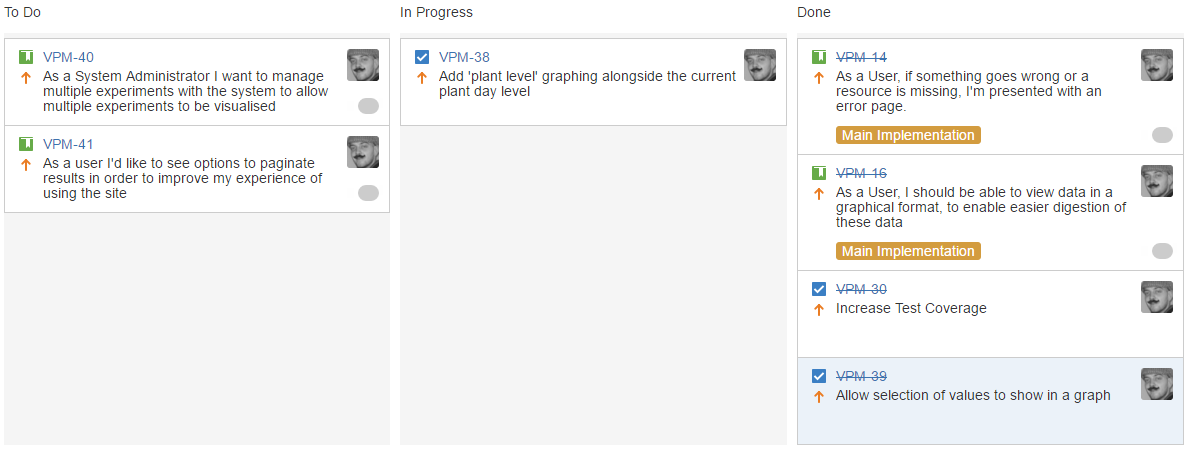
\includegraphics[width=\textwidth]{images/tools/sprint1}
    \caption{A screenshot showing part the current sprint screen in Jira}
    \label{fig:jira_sprint}
\end{figure} 

 Bugs could also be tracked as issues within Jira and added to the current sprint if necessary, I found this to be a valuable way to deal with emergent issues during development as it allowed a simple way to assign priority to urgent issues and keep track of less usgent bugs in the project backlog to be worked on in a future sprint. Figure \ref{fig:jira_bugs} shows a selection of bugs raised as part of development, Jira provides simple methods for filtering all issues against a project by type or status allowing quick access to screens such as this.

\begin{figure}[H]
    \centering
    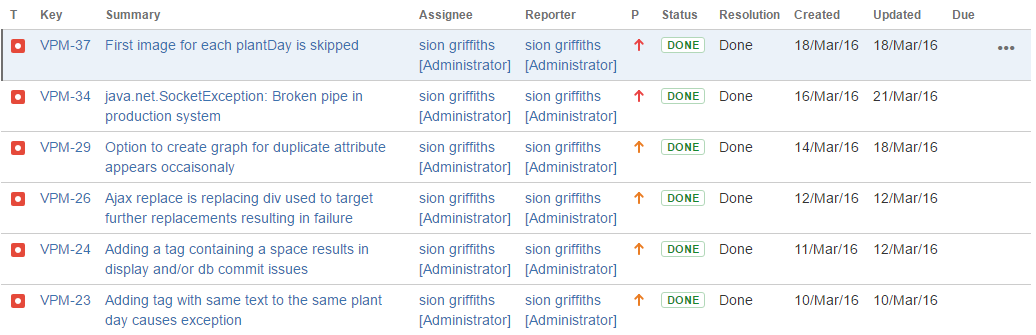
\includegraphics[width=\textwidth]{images/tools/jira_bugs}
    \caption{A screenshot showing version control commit tracking within Jira}
    \label{fig:jira_bugs}
\end{figure} 

Another helpful feature was the integration with the version control repository hosted on Github. Referencing the issue ID in Jira in a commit message linked the commits with the issue within Jira. This provided a handy way to track development against particular issues over time and allowed a quick way to navigate between the issues in Jira and the commits on Github. 

\begin{figure}[H]
    \centering
    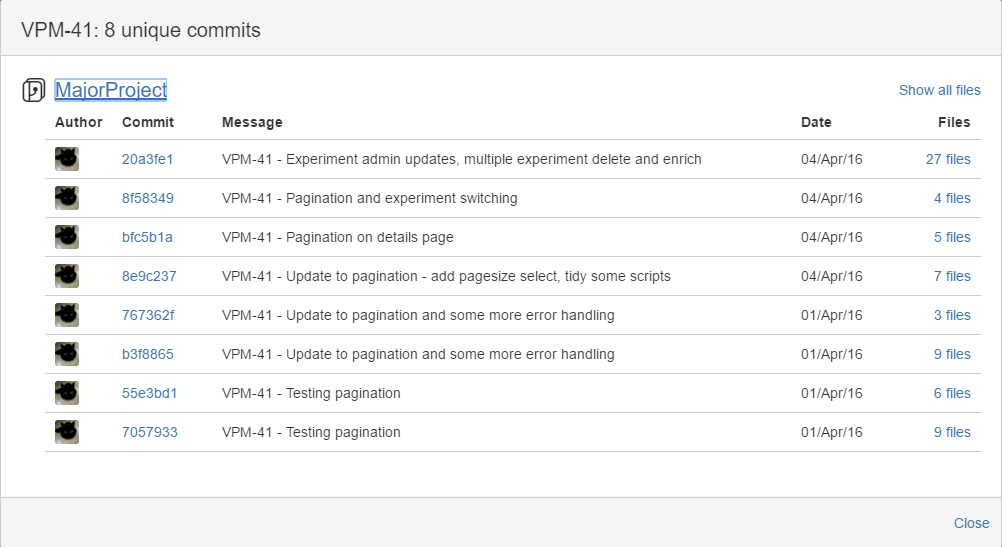
\includegraphics[width=\textwidth]{images/tools/jira_commit}
    \caption{A screenshot showing version control commit tracking within Jira}
    \label{fig:jira_commit}
\end{figure} 

There are a vast array of alternatives that could have been used for issue tracking within the project, many provide the full array of features that were used in Jira during the development of this project. However, Jira being the industry leader, provided an opportunity to gain further valuable experience of its use in a day to day, agile development project. Having previously been involved in the running of a Jira system during my time in industry provided me with familiarisation in configuring a project for my needs and confidence in being able to do so quickly. This was enough to chose Jira over the alternatives that were evaluated such as Waffle.io and the native issue tracking feature provided with Github.

\subsection{Codeship} 
Codeship\cite{_codeship} is a web based Continuous Integration(CI) service. Working in conjunction with the version control repository, Codeship will detect up any commits made to the repository hosted on Github and execute build and test scripts defined as part of the initial setup of the CI service. Use of a CI system within the project provided assurance that each incremental change made to the system integrated correctly and that all tests continued to pass. A notification would be sent in the event of build or test failure.  

 The build script for the project can be seen in figure~\ref{fig:build_script} showing how the project databases are setup and the environment is configured prior to executing the project build and test commands.

 The scripts are invoked within small Docker \cite{docker} based environments which allow build dependencies to be modularised and configured quickly. The initial integration of the CI system into the project environment was extremely simple, linking the Github repository for the project was a couple of mouse clicks and the script below is the entirety of the extra configuration required to get the CI system fully up and running. 

It was because of this speed and simplicity of configuration that Codeship was chosen over rival offerings such as TravisCI \cite{travis} which appeared to have a much more complex initial setup during evaluation.

\begin{figure}[H]
    \centering
    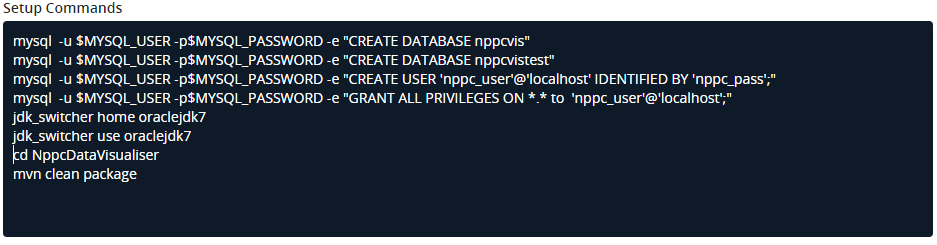
\includegraphics[width=\textwidth]{images/tools/codeShipScript}
    \caption{The project build script on Codeship}
    \label{fig:build_script}
\end{figure} 

\begin{figure}[H]
    \centering
    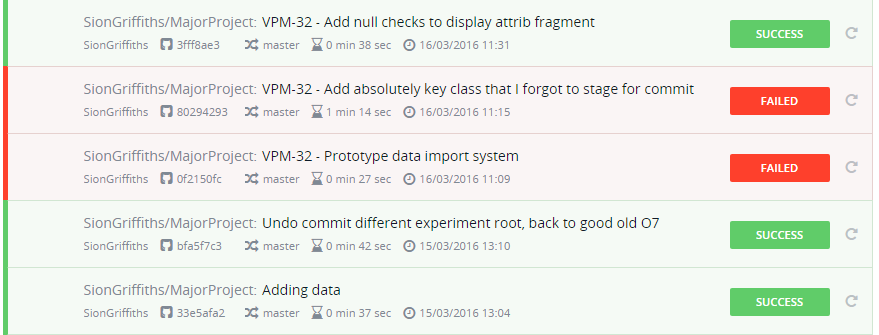
\includegraphics[width=\textwidth]{images/tools/codeShipSmall}
    \caption{A sample of the build history in Codeship}
    \label{fig:build_history}
\end{figure} 



\subsection{Maven}

\section{Some detailed design}

\subsection{Even more detail}

\section{User Interface}

\section{Other relevant sections}